\newcommand{\malwareResultsAucTable}{
    \begin{table}[H]
        \centering
        \begin{tabular}{|p{2,4cm}||P{3,2cm} P{3,2cm} P{3,2cm}|}
            \hline
            Malware Label & ALOHA (M/B only) & ALOHA & Proposed Model \\
            \hline
            AUC-ROC & 0.995$\pm$0.000 & 0.995$\pm$0.001 & \textBF{0.996$\pm$0.001} \\
            \hline
        \end{tabular}
        \caption[Malware Label prediction task AUC-ROC results]{AUC-ROC (Area Under Curve) of the different models for the \textbf{Malware Label} prediction task. Results were aggregated over \textBF{3} training runs with different weight initializations and minibatch orderings. Best results are shown in \textbf{bold}.} \label{tab:malware_auc}
    \end{table}
}

\newcommand{\malwareResultsAtFprTable}{
    \begin{center}
        \begin{longtable}[c]{|P{3,2cm}||P{1,8cm} P{1,8cm} P{1,8cm} P{1,8cm} P{1,8cm}|}
            \hline
            Malware Label & \multicolumn{5}{c|}{{FPR}} \\
            & $10^{-5}$ & $10^{-4}$ & $10^{-3}$ & $10^{-2}$ & $10^{-1}$ \\
            \hline
            \endfirsthead

            \caption*{\raggedright ...continued from previous page} \\
            \hline
            Malware Label & \multicolumn{5}{c|}{\textbf{FPR}} \\
            & $10^{-5}$ & $10^{-4}$ & $10^{-3}$ & $10^{-2}$ & $10^{-1}$ \\
            \hline
            \endhead

            \caption*{\raggedleft ...continued on next page} \\
            \endfoot

            \caption[Malware Label prediction task results]{Mean and standard deviation results (TPR, Accuracy, Recall, Precision and F1-Score) of the different models for the \textbf{Malware Label} prediction task at different \textbf{FPR}s (\textit{False Positive Rates}). Results were aggregated over \textBF{3} training runs with different weight initializations and minibatch orderings. Best results are shown in \textbf{bold}. Under \textbf{TPR} results are also presented the percentage reduction in mean detection error and in ROC curve standard deviation introduced by the \textit{Proposed Model} with respect to both \textit{ALOHA} model and \textit{Joint Embedding}.} \label{tab:malware_results_at_fpr} \\
            \endlastfoot

            \multicolumn{6}{|c|}{\textbf{TPR}} \\
            \hline
            ALOHA (M/B only) & 0.215$\pm$0.032 & 0.647$\pm$0.033 & 0.883$\pm$0.005 & 0.959$\pm$0.003 & 0.990$\pm$0.001 \\
            ALOHA & 0.599$\pm$0.023 & 0.790$\pm$0.005 & 0.879$\pm$0.007 & 0.956$\pm$0.011 & 0.990$\pm$0.001 \\
            Proposed Model & \textBF{0.622$\pm$0.058} & \textBF{0.836$\pm$0.007} & \textBF{0.909$\pm$0.001} & \textBF{0.959$\pm$0.001} & \textBF{0.992$\pm$0.001} \\
            \hline
            Error Reduction wrt ALOHA (M/B only) & 51.8\% & 53.5\% & 22.2\% & 0.0\% & 20.0\% \\
            Error Reduction wrt ALOHA & 5.7\% & 21.9\% & 24.8\% & 6.8\% & 20.0\% \\
            \hline
            Std Reduction wrt ALOHA (M/B only) & -81.2\% & 78.8\% & 80.0\% & 66.7\% & 0.0\% \\
            Std Reduction wrt ALOHA & -152.2\% & -40.0\% & 85.7\% & 90.9\% & 0.0\% \\
            \hline
            \multicolumn{6}{|c|}{\textbf{Accuracy}} \\
            \hline
            ALOHA (M/B only) & 0.696$\pm$0.012 & 0.863$\pm$0.013 & 0.954$\pm$0.002 & 0.978$\pm$0.001 & \textBF{0.935$\pm$0.000} \\
            ALOHA & 0.845$\pm$0.009 & 0.919$\pm$0.002 & 0.953$\pm$0.003 & 0.977$\pm$0.004 & \textBF{0.935$\pm$0.000} \\
            Proposed Model & \textBF{0.854$\pm$0.023} & \textBF{0.936$\pm$0.003} & \textBF{0.964$\pm$0.000} & \textBF{0.978$\pm$0.000} & \textBF{0.935$\pm$0.000} \\
            \hline
            \multicolumn{6}{|c|}{\textbf{Recall}} \\
            \hline
            ALOHA (M/B only) & 0.215$\pm$0.032 & 0.647$\pm$0.033 & 0.883$\pm$0.005 & 0.959$\pm$0.003 & 0.990$\pm$0.001 \\
            ALOHA & 0.599$\pm$0.023 & 0.790$\pm$0.005 & 0.879$\pm$0.007 & 0.956$\pm$0.011 & 0.990$\pm$0.001 \\
            Proposed Model & \textBF{0.622$\pm$0.058} & \textBF{0.836$\pm$0.007} & \textBF{0.909$\pm$0.001} & \textBF{0.959$\pm$0.001} & \textBF{0.992$\pm$0.001} \\
            \hline
            \multicolumn{6}{|c|}{\textbf{Precision}} \\
            \hline
            ALOHA (M/B only) & \textBF{1.000$\pm$0.000} & \textBF{1.000$\pm$0.000} & \textBF{0.998$\pm$0.000} & \textBF{0.984$\pm$0.000} & \textBF{0.862$\pm$0.000} \\
            ALOHA & \textBF{1.000$\pm$0.000} & \textBF{1.000$\pm$0.000} & \textBF{0.998$\pm$0.000} & \textBF{0.984$\pm$0.000} & \textBF{0.862$\pm$0.000} \\
            Proposed Model & \textBF{1.000$\pm$0.000} & \textBF{1.000$\pm$0.000} & \textBF{0.998$\pm$0.000} & \textBF{0.984$\pm$0.000} & \textBF{0.862$\pm$0.000} \\
            \hline
            \multicolumn{6}{|c|}{\textbf{F1 Score}} \\
            \hline
            ALOHA (M/B only) & 0.353$\pm$0.043 & 0.785$\pm$0.024 & 0.937$\pm$0.003 & 0.971$\pm$0.001 & 0.921$\pm$0.000 \\
            ALOHA & 0.749$\pm$0.018 & 0.883$\pm$0.003 & 0.935$\pm$0.004 & 0.970$\pm$0.006 & \textBF{0.922$\pm$0.000} \\
            Proposed Model & \textBF{0.765$\pm$0.044} & \textBF{0.911$\pm$0.004} & \textBF{0.952$\pm$0.001} & \textBF{0.971$\pm$0.000} & 0.922$\pm$0.001 \\
            \hline
        \end{longtable}
    \end{center}
}

\newcommand{\malwareResultsSummaryTable}{
    \begin{table}[H]
        \centering
        \begin{tabular}{|P{3,2cm}||P{1,8cm} P{1,8cm} P{1,8cm} P{1,8cm} P{1,8cm}|}
            \hline
            \multicolumn{6}{|c|}{Malware Label (at FPR $=1\%$)} \\
            \hline
            Model & TPR & Accuracy & Precision & Recall & F1 score \\
            \hline
            ALOHA (M/B only) & 0.959$\pm$0.003 & 0.978$\pm$0.001 & \textBF{0.984$\pm$0.000} & 0.959$\pm$0.003 & 0.971$\pm$0.001 \\
            ALOHA & 0.956$\pm$0.011 & 0.977$\pm$0.004 & \textBF{0.984$\pm$0.000} & 0.956$\pm$0.011 & 0.970$\pm$0.006 \\
            Proposed Model & \textBF{0.959$\pm$0.001} & \textBF{0.978$\pm$0.000} & \textBF{0.984$\pm$0.000} & \textBF{0.959$\pm$0.001} & \textBF{0.971$\pm$0.000} \\
            \hline
        \end{tabular}
        \caption[Summary of Malware Label prediction task results]{Summary of the mean and standard deviation results of the different models for the \textbf{Malware Label} prediction task at \textbf{FPR} $=1\%$. Results were aggregated over \textBF{3} training runs with different weight initializations and minibatch orderings. Best results are shown in \textbf{bold}.} \label{tab:malware_result_summary}
    \end{table}
}

\newcommand{\malwareRocAlohaMB}{
    \begin{figure}[H]
        \vspace*{-0.5cm}
        \centering
        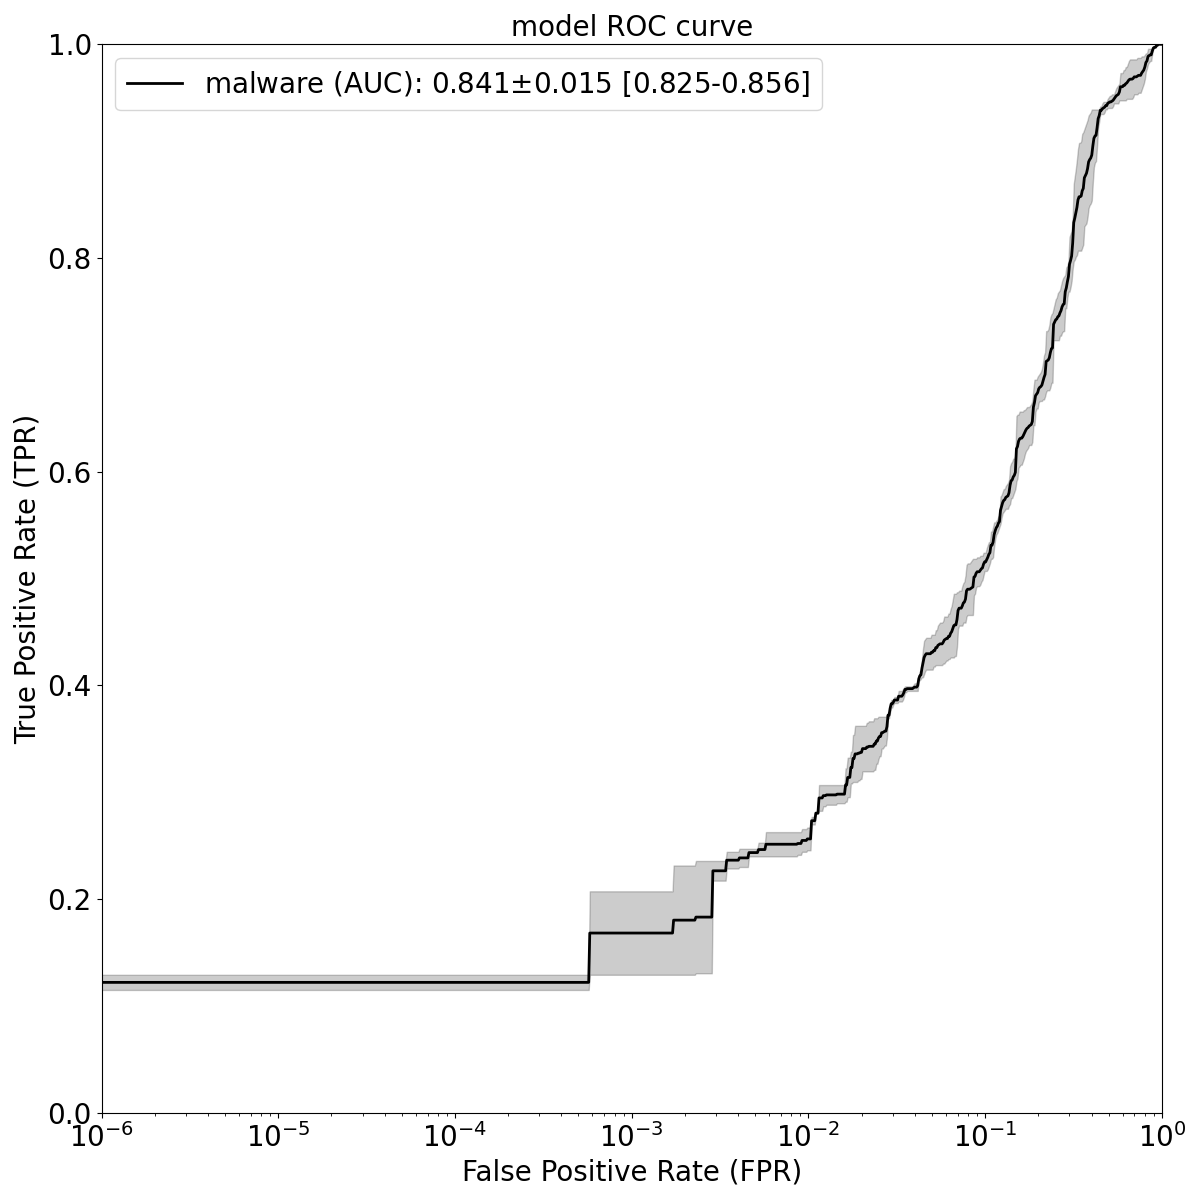
\includegraphics[width=0.7\textwidth]{./results/malware_roc_alohaMB.png}
        \vspace*{-0.2cm}
        \caption[Malware Label prediction task ALOHA (M/B only) ROC curve]{ROC curve and AUC statistics of \textBF{ALOHA (M/B only)} model for the \textbf{Malware Label}. The line represents the \textit{mean} TPR at a given FPR, while the shaded region represents the \textit{standard deviation}. Statistics were computed over \textBF{3} training runs, each with random parameter initialization.}
        \label{fig:malwareRocAlohaMB}
    \end{figure}
}

\newcommand{\malwareRocAloha}{
    \begin{figure}[H]
        \vspace*{-0.5cm}
        \centering
        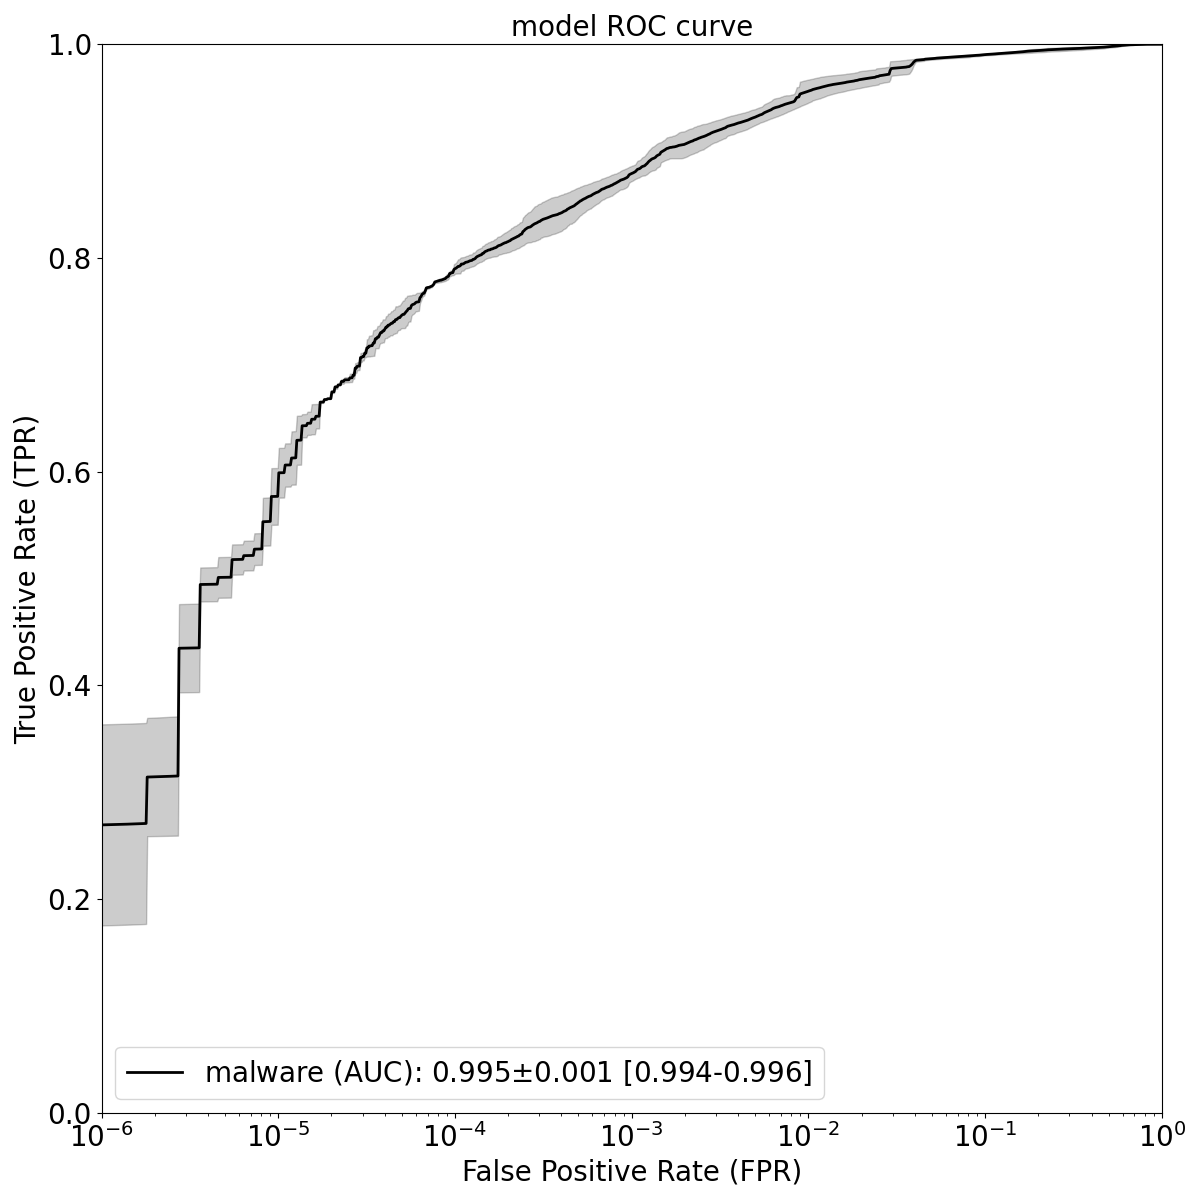
\includegraphics[width=0.7\textwidth]{./results/malware_roc_aloha.png}
        \vspace*{-0.2cm}
        \caption[Malware Label prediction task ALOHA ROC curve]{ROC curve and AUC statistics of \textBF{ALOHA} model for the \textbf{Malware Label}. The line represents the \textit{mean} TPR at a given FPR, while the shaded region represents the \textit{standard deviation}. Statistics were computed over \textBF{3} training runs, each with random parameter initialization.}
        \label{fig:malwareRocAloha}
    \end{figure}
}

\newcommand{\malwareRocProposedMethod}{
    \begin{figure}[H]
        \vspace*{-0.5cm}
        \centering
        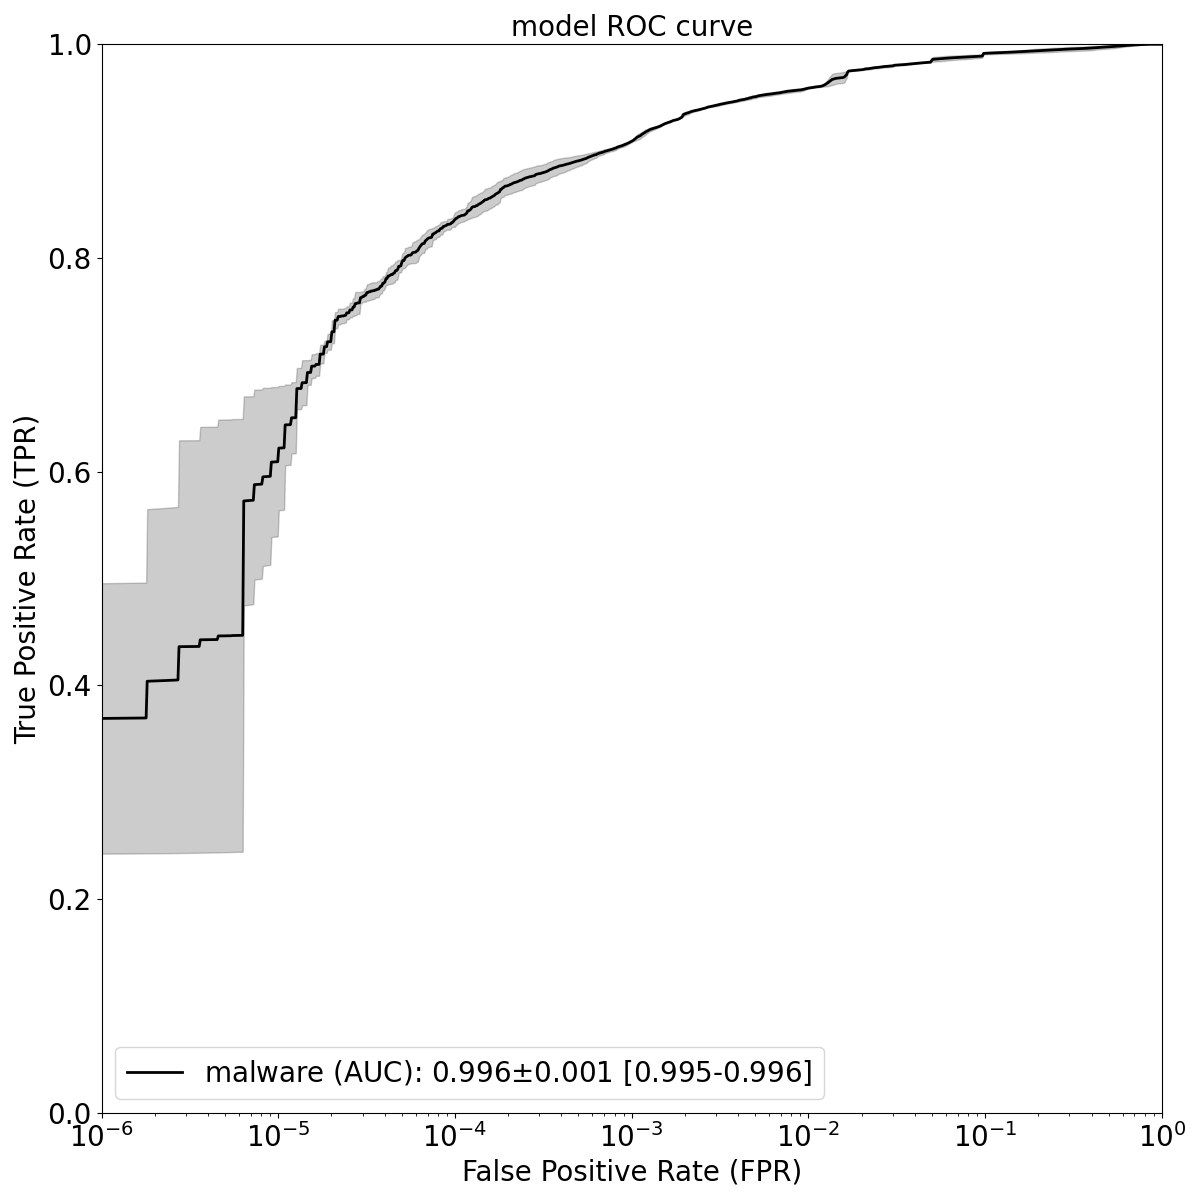
\includegraphics[width=0.7\textwidth]{./results/malware_roc_proposedModel.png}
        \vspace*{-0.2cm}
        \caption[Malware Label prediction task Proposed Model ROC curve]{ROC curve and AUC statistics of \textBF{Proposed Model} for the \textbf{Malware Label}. The line represents the \textit{mean} TPR at a given FPR, while the shaded region represents the \textit{standard deviation}. Statistics were computed over \textBF{3} training runs, each with random parameter initialization.}
        \label{fig:malwareRocProposedModel}
    \end{figure}
}
